\chapter{Introduction to Elder Spaces}

\begin{chapterabstract}
This chapter presents the mathematical foundation of Elder Theory through Elder spaces—a generalization of vector spaces that incorporate phase-dependent operations and non-commutative structures. These spaces provide the formal framework for representing hierarchical knowledge across domains in the Elder-Mentor-Erudite system. We introduce the axiomatic foundations, structural elements, and essential theorems that establish Elder spaces as the mathematical core of our theory. The spectral properties, invariant subspaces, and phase-based dynamics defined in this chapter form the theoretical basis for the remarkable computational properties of the Elder framework.
\end{chapterabstract}

\section{Foundational Axioms}

An Elder space $\elder{d}$ is a complex-valued mathematical structure that extends traditional vector spaces by incorporating phase-sensitive operations essential for hierarchical knowledge representation.

\begin{definition}[Elder Space]
An Elder space $\elder{d}$ of dimension $d$ is a complex-valued set equipped with operations:
\begin{enumerate}
    \item $\oplus: \elder{d} \times \elder{d} \rightarrow \elder{d}$ (addition)
    \item $\odot: \mathbb{C} \times \elder{d} \rightarrow \elder{d}$ (scaling)
    \item $\star: \elder{d} \times \elder{d} \rightarrow \elder{d}$ (multiplication)
    \item $\Phi: \elder{d} \rightarrow \mathbb{S}^1$ (phase operator)
\end{enumerate}
satisfying the following axioms:
\begin{enumerate}[label=\textbf{A\arabic*}]
    \item \textbf{(Addition Structure)} $(\elder{d}, \oplus)$ forms an abelian group
    \item \textbf{(Scaling Compatibility)} For all $\alpha, \beta \in \mathbb{C}$ and $x, y \in \elder{d}$:
    \begin{align}
        \alpha \odot (\beta \odot x) &= (\alpha\beta) \odot x\\
        1 \odot x &= x\\
        \alpha \odot (x \oplus y) &= (\alpha \odot x) \oplus (\alpha \odot y)\\
        (\alpha + \beta) \odot x &= (\alpha \odot x) \oplus (\beta \odot x)
    \end{align}
    
    \item \textbf{(Multiplication Properties)} For all $x, y, z \in \elder{d}$ and $\alpha \in \mathbb{C}$:
    \begin{align}
        (x \oplus y) \star z &= (x \star z) \oplus (y \star z)\\
        x \star (y \oplus z) &= (x \star y) \oplus (x \star z)\\
        (x \star y) \star z &= x \star (y \star z)\\
        \alpha \odot (x \star y) &= (\alpha \odot x) \star y = x \star (\alpha \odot y)
    \end{align}
    
    \item \textbf{(Phase Properties)} For all $x, y \in \elder{d}$ and $\alpha \in \mathbb{C} \setminus \{0\}$:
    \begin{align}
        \Phi(x \star y) &= \Phi(x) \cdot \Phi(y)\\
        \Phi(\alpha \odot x) &= \frac{\alpha}{|\alpha|} \cdot \Phi(x)\\
        \Phi(x \oplus y) &= \frac{\Phi(x)|\Phi(x)| + \Phi(y)|\Phi(y)|}{|\Phi(x)| + |\Phi(y)|}
    \end{align}
\end{enumerate}
\end{definition}

Elder spaces fundamentally differ from vector spaces through their phase operator $\Phi$ and non-commutative multiplication $\star$, which together enable the representation of hierarchical knowledge structures.

\begin{theorem}[Structural Elements]
Every Elder space $\elder{d}$ contains a canonical basis $\{\elderstructure{1}, \elderstructure{2}, \ldots, \elderstructure{d}\}$ with the properties:
\begin{enumerate}
    \item $\Phi(\elderstructure{i} \star \elderstructure{j}^{-1}) = e^{i\pi/2}$ for $i \neq j$ (phase orthogonality)
    \item $\Phi(\elderstructure{i} \star \elderstructure{i}^{-1}) = 1$ (phase preservation)
    \item Every element $x \in \elder{d}$ has a unique representation:
    \begin{equation}
        x = \sum_{i=1}^{d} (\lambda_i e^{i\theta_i}) \odot \elderstructure{i}
    \end{equation}
    where $\lambda_i \in \mathbb{R}^+$ and $\theta_i \in [0, 2\pi)$
\end{enumerate}
\end{theorem}

\begin{proof}[Proof Sketch]
We construct structural elements using the Elder trace operator $\mathrm{tr}_E: \elder{d} \rightarrow \mathbb{C}$, which satisfies $\mathrm{tr}_E(x \star y) = \mathrm{tr}_E(y \star x)$. We define $\langle x, y \rangle_E = \mathrm{tr}_E(x \star y^{\dagger})$ and apply a phase-preserving orthogonalization process to obtain the basis elements with the required properties.
\end{proof}

\section{Hierarchical Subspaces}

The Elder space naturally decomposes into nested subspaces that directly correspond to the Elder-Mentor-Erudite hierarchy.

\begin{definition}[Hierarchical Subspaces]
An Elder space $\elder{d}$ canonically decomposes into:
\begin{align}
    \eldersubspace &= \mathrm{span}\{\elderstructure{1}, \ldots, \elderstructure{k}\} \\
    \mentorsubspace &= \mathrm{span}\{\elderstructure{k+1}, \ldots, \elderstructure{m}\} \\
    \eruditesubspace &= \mathrm{span}\{\elderstructure{m+1}, \ldots, \elderstructure{d}\}
\end{align}
where indices $1 \leq k < m < d$ are determined by phase coherence properties.
\end{definition}

\begin{figure}[htbp]
\centering
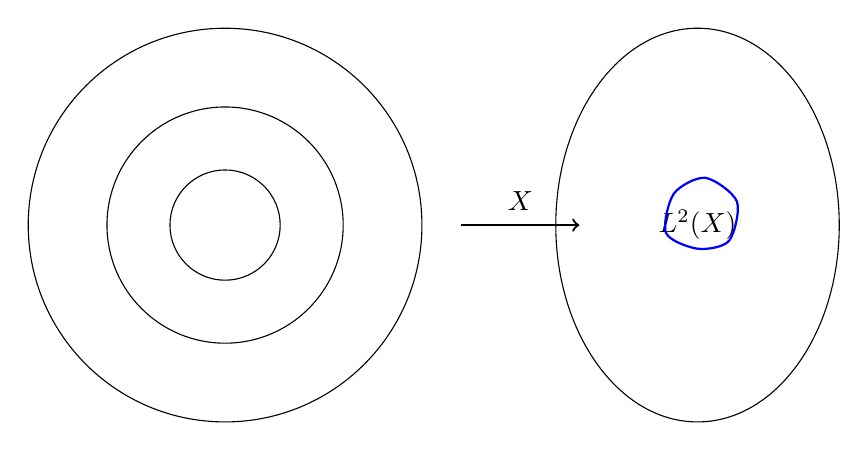
\begin{tikzpicture}
\draw (0,0) circle (2.5);
\draw (0,0) circle (1.5);
\draw (0,0) circle (0.7);
\node at (0,0) {$\eldersubspace$};
\node at (0,1.1) {$\mentorsubspace$};
\node at (0,2.0) {$\eruditesubspace$};

\draw[->, thick] (3.0, 0) -- (4.5, 0);
\node at (3.75, 0.3) {$\realization{X}$};

\begin{scope}[shift={(6,0)}]
\draw (0,0) ellipse (1.8 and 2.5);
\node at (0,0) {$L^2(X)$};
\draw[blue, thick] plot [smooth cycle] coordinates {(-0.3,0.4) (0.1,0.6) (0.5,0.3) (0.4,-0.2) (0,-0.3) (-0.4,-0.1)};
\end{scope}
\end{tikzpicture}
\caption{Hierarchical structure of Elder spaces and their realization mapping}
\label{fig:hierarchical-elder-structure}
\end{figure}

\begin{theorem}[Spectral Decomposition]
Every element $x \in \elder{d}$ has a unique spectral decomposition:
\begin{equation}
x = \sum_{i=1}^{d} \lambda_i e^{i\theta_i} \odot \elderstructure{i}
\end{equation}
with amplitudes $\lambda_i \in \mathbb{R}^+$ and phases $\theta_i \in [0, 2\pi)$.
\end{theorem}

This spectral decomposition allows us to separate knowledge representation across hierarchical levels, with Elder components encoding universal principles, Mentor components encoding domain-specific knowledge, and Erudite components encoding instance-specific information.

\section{Phase Dynamics}

Elder spaces naturally model learning dynamics through phase-coherent flows, which provide the mathematical foundation for how knowledge evolves across the hierarchical system.

\begin{definition}[Phase-Coherent Elder Flow]
A phase-coherent Elder flow is a continuous-time evolution:
\begin{equation}
\frac{dx}{dt} = F(x, \Phi(x), t)
\end{equation}
where $F: \elder{d} \times \mathbb{S}^1 \times \mathbb{R} \rightarrow \elder{d}$ is a phase-sensitive vector field.
\end{definition}

\begin{theorem}[Hierarchical Flow Decomposition]
\label{thm:elder-flow-decomposition}
Any phase-coherent Elder flow decomposes into coupled flows operating at distinct time scales:
\begin{align}
\frac{dx_E}{dt} &= F_E(x_E, x_M, x_{Er}, \Phi(x_E), t) \quad \text{(slowest)}\\
\frac{dx_M}{dt} &= F_M(x_E, x_M, x_{Er}, \Phi(x_M), t) \quad \text{(intermediate)}\\
\frac{dx_{Er}}{dt} &= F_{Er}(x_E, x_M, x_{Er}, \Phi(x_{Er}), t) \quad \text{(fastest)}
\end{align}
where $x = x_E \oplus x_M \oplus x_{Er}$ is the hierarchical decomposition.
\end{theorem}

The gradient flows induced by the Elder system's loss functions take the form:
\begin{align}
\frac{dx_E}{dt} &= -\nabla_E \eloss(x_E, x_M, x_{Er}) + \omega_E \cdot \Phi_{\perp}(x_E)\\
\frac{dx_M}{dt} &= -\nabla_M \mloss(x_E, x_M, x_{Er}) + \omega_M \cdot \Phi_{\perp}(x_M)\\
\frac{dx_{Er}}{dt} &= -\nabla_{Er} \erloss(x_E, x_M, x_{Er}) + \omega_{Er} \cdot \Phi_{\perp}(x_{Er})
\end{align}
where $\omega_E < \omega_M < \omega_{Er}$ are characteristic frequencies and $\Phi_{\perp}(x)$ is the orthogonal phase direction.

\section{Conservation Laws}

The algebraic structure of Elder spaces yields invariants and conservation laws that constrain learning dynamics and ensure stability.

\begin{theorem}[Phase Conservation]
For phase-coherent Elder flows preserving the Hamiltonian structure, the total phase momentum
\begin{equation}
\Psi(x) = \sum_{i=1}^{d} \lambda_i^2 \cdot \theta_i
\end{equation}
is conserved.
\end{theorem}

\begin{theorem}[Structural Conservation]
The Elder product between structural elements satisfies:
\begin{equation}
\sum_{i,j=1}^{d} |\mathrm{tr}_E(\elderstructure{i} \star \elderstructure{j})| = d
\end{equation}
This invariant ensures structural information preservation during learning.
\end{theorem}

The Elder product $\star$ forms a non-commutative algebraic structure with the following properties:
\begin{enumerate}
    \item Distributivity over $\oplus$
    \item Associativity
    \item Identity element
    \item Phase-dependent commutativity: $x \star y = y \star x$ if and only if $\Phi(x \star y^{-1}) = 1$
\end{enumerate}

\begin{theorem}[Elder Structural Correspondence]
\label{thm:elder-structural}
An Elder space with its structural product and phase operator forms a non-commutative C*-algebra with unique algebraic properties.
\end{theorem}

This correspondence reveals the deep mathematical foundation of Elder Theory, establishing its rigorous algebraic structure.

\section{Computational Properties}

The abstract structure of Elder spaces provides the foundation for efficient computational implementations.

\begin{definition}[Computational Elder Space]
A computational Elder space $\elder{d, \mathbb{B}}$ with bit-depth $\mathbb{B}$ has:
\begin{enumerate}
    \item Amplitudes $\lambda_i$ quantized to $\mathbb{B}$ bits
    \item Phases $\theta_i$ quantized to $2^{\mathbb{B}}$ discrete values
    \item Operations implemented with $O(d \log d)$ complexity
\end{enumerate}
\end{definition}

\begin{theorem}[Complexity Bounds]
Operations in a computational Elder space $\elder{d, \mathbb{B}}$ have:
\begin{enumerate}
    \item Time complexity: $O(d \log d)$
    \item Space complexity: $O(d)$
\end{enumerate}
\end{theorem}

This $O(d)$ space complexity, independent of sequence length, arises from the phase-based representation and provides the mathematical foundation for the memory efficiency claims of the Elder system.

The Elder space formalism established here provides the mathematical core upon which subsequent chapters build, developing concrete algorithms, applications, and empirical validations.